\chapter{Logging}
\label{sec:module.Logging}
F�r eine gr�ndliche Analyse der Spiele sind ausf�hrliche und konfigurierbare Logfiles unabdingbar. Zu diesem Zweck haben wir bereits im Rahmen des ''Projekts 2 `` ein flexibles Logging-Framework geschrieben. Dieses Framework haben wir im Rahmen der Bachelorarbeit noch einmal verbessert und erweitert. Auch die Auslagerung in eine separates, unabh�ngiges Modul geschah im Rahmen der Bachelorarbeit.

\begin{figure}[H]
\centering
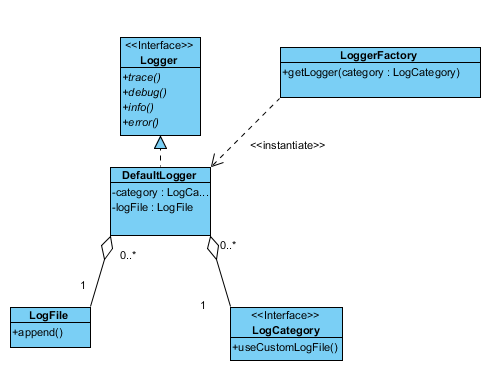
\includegraphics[width=0.8\textwidth]{91_bilder/Logging}
\caption{Logging Klassen}
\label{fig:Logging}
\end{figure}

Abbildung \ref{fig:Logging} zeigt die wichtigsten Klassen des Logging-Frameworks. 
\begin{itemize}
\item
\textbf{Logger:} Das Logger Interface definiert die Methoden, die aus dem Applikations-Code heraus zum Logging verwendet werden k�nnen. Die Methodennamen (\texttt{debug(...)},\texttt{error(...)} etc.) bezeichnen den LogLevel, als Argumente �bergeben werden ein String mit der Logmeldung sowie eine Liste von zus�tzlichen Parametern, die in die Logmeldung eingef�gt werden soll. Die Methoden unterst�tzen alle die Java String Formatter Syntax. \footnote{\url{http://docs.oracle.com/javase/6/docs/api/java/util/Formatter.html\#syntax}}
\item
\textbf{DefaultLogger:} Unsere Standardimplementierung des Logger Interfaces. Der DefaultLogger hat jeweils eine LogCategory und ein LogFile, in das er seine Meldungen schreibt.
\item
\textbf{LogFile:} Das LogFile ist f�r eine einzelne Log-Datei zust�ndig; alle Logger, die in eine bestimmte Log-Datei schreiben wollen, greifen auf dieselbe LogFile Instanz zu. Die ''physische`` Datei auf dem Dateisystem wird von der LogFile Instanz erst erstellt, wenn die erste Log-Meldung geschrieben werden soll.
\item
\textbf{LogCategory:} Jede Log-Meldung geh�rt zu einer Kategorie. Dieses Interface bietet den verwendenden Modulen die M�glichkeit, eigene Kategorien zu definieren; das Logging-Framework selber definiert keine Kategorien. Mit der Methode useCustomLogFile() kann f�r eine Kategorie bestimmt werden, ob sie in das globale LogFile oder ein eigenes loggt. Dadurch kann die \"Ubersichtlichkeit in den Log-Dateien gesteigert werden.
\item
\textbf{LoggerFactory:} S�mtliches Erstellen von Logger-Instanzen l�uft �ber die LoggerFactory. Sie stellt sicher, dass LogFile-Instanzen wiederverwendet werden und erstellt jeweils einen passenden Logger.
\end{itemize}

\section{Konfiguration}
\label{sec:module.Logging.Konfiguration}

\begin{figure}[H]
\centering
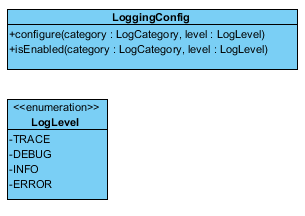
\includegraphics[width=0.5\textwidth]{91_bilder/LoggingConfig}
\caption{Logging Konfiguration}
\label{fig:LoggingConfig}
\end{figure}

Abbildung \ref{fig:LoggingConfig} zeigt die Konfigurations-Klassen des Logging-Frameworks. Mit der Methode \texttt{configure()} der Klasse LoggingConfig kann der LogLevel f�r eine bestimmte Kategorie eingestellt werden. Mit der Methode \texttt{isEnabled()} kann abgefragt werden, ob ein bestimmter LogLevel f�r eine bestimmte Kategorie aktiv ist.

Der LogLevel bestimmt, ob eine Meldung �berhaupt ins Log geschrieben wird. Die LogLevel haben eine implizite Hierarchie, wie man das von verbreiteteren Logging-Frameworks (z.B. Log4j, SLF4J) her kennt: TRACE > DEBUG > INFO > ERROR. Das heisst, wenn f�r eine Kategorie der LogLevel INFO definiert ist, werden Meldungen mit Level INFO und ERROR geloggt, DEBUG und TRACE aber nicht. Auf diese Weise ist eine feingranulare Kontrolle dar�ber m�glich, was genau geloggt wird und was nicht.

\section{Anwendungsbeispiele}
\label{sec:module.Logging.Beispiele}

Folgende Codezeilen zeigen, wie drei Log-Kategorien mit unterschiedlichen LogLevels konfiguriert werden k�nnen:
\lstset{language=Java, tabsize=4}
\begin{lstlisting}
LoggingConfig.configure(LogCategory.ORDERS, LogLevel.DEBUG);
LoggingConfig.configure(LogCategory.PERFORMANCE, LogLevel.TRACE);
LoggingConfig.configure(LogCategory.SETUP, LogLevel.ERROR);
\end{lstlisting}

Folgende Codezeilen zeigen, wie ein Logger instanziert wird:
\lstset{language=Java, tabsize=4}
\begin{lstlisting}
private static final Logger LOGGER = LoggerFactory.getLogger(LogCategory.ATTACK_HILLS);
\end{lstlisting}

Folgende Codezeilen zeigen, wie ein Logger verwendet wird:
\lstset{language=Java, tabsize=4}
\begin{lstlisting}
LOGGER.info("AttackHillMission:new ants gathered for hill %s amount %s Ants: %s", enemyHill, newAnts.size(),
                newAnts.keySet());
\end{lstlisting}


\section{JavaScript Addon f�r HMTL-Gameviewer}
\label{sec:module.Logging.Addon}
Das Codepaket welches von den Challenge-Organisatoren mitgeliefert wird, bietet bereits eine hilfreiche 2D-Visualisierung des Spiels, mit welchem das Spielgeschehen mitverfolgt werden kann. Die Visualisierung wurde mit HMTL und Javascript implementiert. Leider ist es nicht m�glich zus�tzliche Informationen auf die Seite zu projizieren. Deshalb haben wir den Viewer bereits im Projekt 2 mit einer solchen Funktion erweitert. Mit der Codezeile LiveInfo.liveInfo(...) kann eine Zusatzinformation geschrieben werden, welche auf dem Viewer sp�ter sichtbar ist. Es muss definiert werden mit welchem Zug und wo auf dem Spielfeld die Information angezeigt werden soll. Im Beispiel wird an der Position der Ameise (ant.getTile()) ausgegeben welchen Task die Ameise hat.
\lstset{language=Java, tabsize=4}
\begin{lstlisting}
LiveInfo.liveInfo(Ants.getAnts().getTurn(), ant.getTile(), 
                "Task: %s ant: %s", issuer, ant.getTile());
\end{lstlisting}
Auf der Karte wird ein einfaches aber praktisches Popup mit den geschriebenen Informationen angezeigt. Dank solcher Zusatzinformationen muss nicht m�hsam im Log nachgeschaut werden, welcher Ameise wann und wo welcher Task zugeordnet ist.

\begin{figure}[H]
\centering
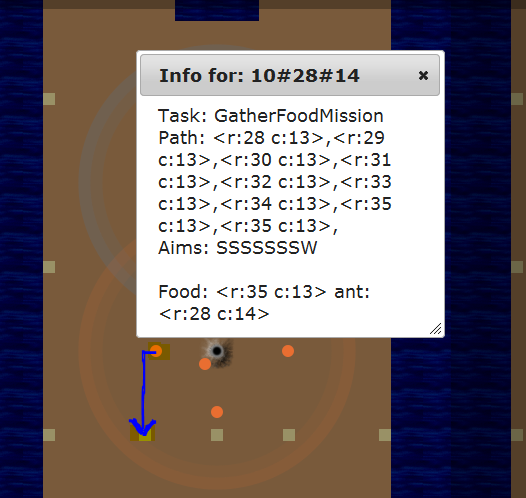
\includegraphics[height=70mm]{91_bilder/javascriptAddon.png}
\caption[Live-Info Popupfenster]{Im Popupfenster steht die Aufgabe der Ameise sowie die Pixel des Pfades (falls vorhanden), welcher die Ameise ablaufen wird.}
\label{fig:javascriptAddon}
\end{figure}


Das angezeigte Popup zeigt welchen Task (GatherFoodTask) die Ameise hat, wo sie sich befindet <r:28 c:14>, welches Futterzelle angesteuert wird <r:35 c:13> und welchen Pfad dazu berechnet wurde.\\Im Rahmen der Bachelorarbeit wurde dieses Addon erweitert. Nun werden alle Pixel welche in dem Popup ausgegeben werden auf der Karte markiert. (Siehe Abb \ref{fig:javascriptAddonPath})

\begin{figure}[H]
\centering
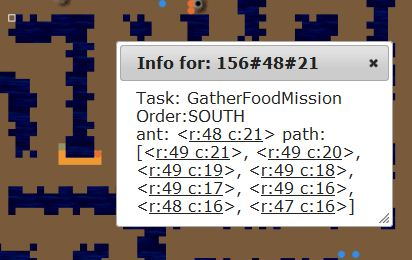
\includegraphics[height=45mm]{91_bilder/javascriptAddon2.jpg}
\caption[Erweiterung des Live-Info Popupfenster]{Mit der erweiterten Version wird der Pfad (orange) der Ameise von <r:48 c:21> nach <r:47 c:16> auf der Karte abgebildet.}
\label{fig:javascriptAddonPath}
\end{figure}


\section{Profile und Logging}
\label{sec:module.Logging.Profile}
Mit der Einf�hrung der Profile gewannen wir die M�glichkeit, mehrere Kopien unseres Bots mit unterschiedlichen Konfigurationen gegeneinander antreten zu lassen. Dazu mussten wir aber die Logfiles so voneinander trennen, dass die Logs der verschiedenen Bots isoliert sind. Die Logfiles werden daher neu in ein Unterverzeichnis mit dem Namen des konfigurierten Profils geschrieben.

F�r das LiveInfo Log, das f�r das Javascript Addon geschrieben wird, verzichteten wir auf eine solche Erweiterung, da so viel Information f�r mehrere Bots nur schwer �bersichtlich darzustellen w�re. Stattdessen bauten wir einen Schalter in den Code ein, mit dem das LiveInfo vor�bergehend deaktiviert werden kann, um Konflikte zwischen den Bots zu vermeiden.